\chapter{Introducció}

L'objectiu principal d'aquest informe és l'estudi de l'aerodinàmica d'un planejador i l'efecte que té sobre ella l'efecte terra.
Es comença analitzant l'aerodinàmica de l'ala aïllada per poder estudiar com influencien els paràmetres geomètrics en l'aerodinàmica, i, un cop determinada la geometria final de l'ala, es procedeix a analitzar l'efecte sòl.

A continuació, s'afegeixen els estabilitzadors vertical i horitzontal i, de nou, se n'estudia els coeficients aerodinàmics. També s'afegeix l'anàlisi de moments. Finalment, es realitza l'anàlisi del planejador complet amb efecte terra.

\begin{figure}[h]
	\centering
	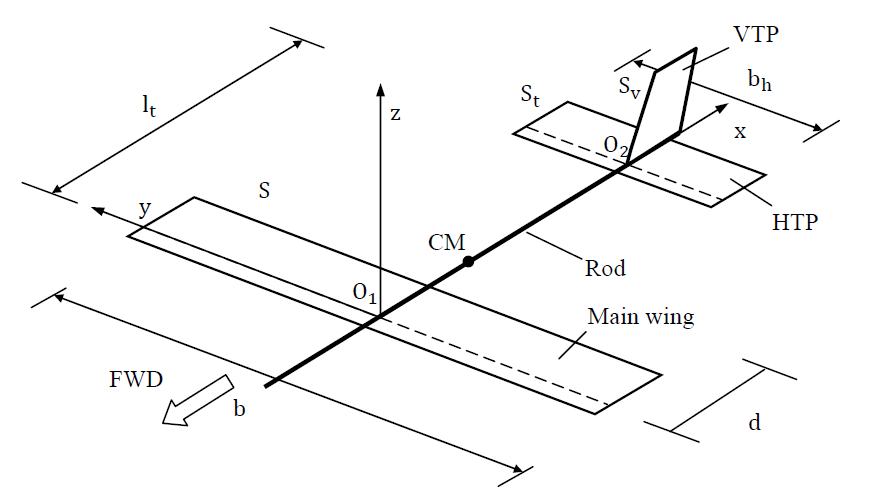
\includegraphics[scale=0.5]{plots/enunciat.png}
	\caption{Esquema del planejador}
	\label{enunciat}
\end{figure}

L'esquema del planejador, així com els paràmetres geomètrics i els eixos de referència utilitzats, es troben definits en la figura \ref{enunciat}. Les relacions entre alguns d'aquests paràmetres estan fixats per les següents expressions:
\begin{itemize}
	\item $\frac{S_{t}}{S}=\frac{1}{8}$
	\item $\frac{S_{v}}{S}=\frac{2}{3}$
	\item $\frac{l_{t}}{\bar{c}}=4$
\end{itemize}

Per tal de definir els paràmetres bàsics de la geometria de l'ala del planejador, s'ha agafat com a referència l'avió SZD-56 Diana 2 de Diana Sailplanes \cite{Kubrynski2006}. Els valors determinats són:
\begin{itemize}
	\item $\lambda=0.3$
	\item $A=26$
	\item $\Lambda=0$
	\item $\Gamma=0$
\end{itemize}
